\documentclass[10pt]{article}
\usepackage[utf8]{inputenc}
\usepackage{mathtools}
\usepackage{amsmath}
\usepackage{graphicx}
\usepackage{array}
\usepackage[margin=0.5in]{geometry}
\usepackage{listings}
\usepackage{color}

\definecolor{mygreen}{rgb}{0,0.6,0}
\definecolor{mygray}{rgb}{0.5,0.5,0.5}
\definecolor{mymauve}{rgb}{0.58,0,0.82}

\lstset{ %
  backgroundcolor=\color{white},   % choose the background color; you must add \usepackage{color} or \usepackage{xcolor}; should come as last argument
  basicstyle=\footnotesize,        % the size of the fonts that are used for the code
  breakatwhitespace=false,         % sets if automatic breaks should only happen at whitespace
  breaklines=true,                 % sets automatic line breaking
  captionpos=b,                    % sets the caption-position to bottom
  commentstyle=\color{mygreen},    % comment style
  deletekeywords={...},            % if you want to delete keywords from the given language
  escapeinside={\%*}{*)},          % if you want to add LaTeX within your code
  extendedchars=true,              % lets you use non-ASCII characters; for 8-bits encodings only, does not work with UTF-8
  frame=single,	                   % adds a frame around the code
  keepspaces=true,                 % keeps spaces in text, useful for keeping indentation of code (possibly needs columns=flexible)
  keywordstyle=\color{blue},       % keyword style
  language=Octave,                 % the language of the code
  morekeywords={*,...},            % if you want to add more keywords to the set
  numbers=left,                    % where to put the line-numbers; possible values are (none, left, right)
  numbersep=5pt,                   % how far the line-numbers are from the code
  numberstyle=\tiny\color{mygray}, % the style that is used for the line-numbers
  rulecolor=\color{black},         % if not set, the frame-color may be changed on line-breaks within not-black text (e.g. comments (green here))
  showspaces=false,                % show spaces everywhere adding particular underscores; it overrides 'showstringspaces'
  showstringspaces=false,          % underline spaces within strings only
  showtabs=false,                  % show tabs within strings adding particular underscores
  stepnumber=2,                    % the step between two line-numbers. If it's 1, each line will be numbered
  stringstyle=\color{mymauve},     % string literal style
  tabsize=2,	                   % sets default tabsize to 2 spaces
  title=\lstname                   % show the filename of files included with \lstinputlisting; also try caption instead of title
}
\renewcommand{\arraystretch}{1.5}
\setcounter{secnumdepth}{0}
\author{Kevin Mambu}
\date{\today}
\title{M1 SESI 2017-2018\\Architecture Multi-Processeurs\\TP7 : Contrôleur DMA}

\begin{document}
\maketitle

\section{A) Objectifs}
Le premier objectif de ce TP est d’analyser le fonctionnement d'un nouveau
contrôleur de périphérique: Le composant IOC (Input Output Controler) peut être
utilisé pour effectuer des transferts de données entre la mémoire et un
périphérique de stockage externe (disque magnétique, clé USB, etc...).

Le second objectif est d'analyser les problèmes posés par le partage des
périphériques quand plusieurs programmes s'exécutent en parallèle sur plusieurs
processeurs, et utilisent le même périphérique. L'architecture matérielle est
donc l'architecture multi-processeurs générique, déjà utilisée dans les TP5,
TP6, et TP7.

\section{B) Contrôleur de disque}
\begin{itemize}
  \item Le composant PibusBlockDevice permet d'acceder à un bloc externe.
  \item LBA : Logic Block Address, numéro de bloc sur un disque.
  \item 1 bloc = 512 octets.
  \item Un accès vers un disque est très long $\rightarrow$ plusieurs millions
  de cycles.
  \item Rôle de l'IOC : déclencher un transfert de données entre le tampon
  mémoire et le disque.
  \item Emulation d'un disque : fichier sotcké sur le disque de la machine hôte.
  \item Fichier \texttt{images.raw} :
  \begin{itemize}
    \item 21 fichiers de 128x128 pixels.
    \item 1 octet = 1 pixel codé sur 256 niveaux de gris.
  \end{itemize}
\end{itemize}

\subsection{Scénario de communication entre \texttt{main} et le contrôleur disque}
\begin{enumerate}
  \item \texttt{main} configure l'IOC via un appel système.
  \item \texttt{main} doit écrire dans les registres mappés en mémoire de l'IOC
  pour lancer le transfert. Il faut spécifier:
  \begin{itemize}
    \item L'adresse de base du tampon mémoire.
    \item Le nombre de blocs à transferer.
    \item Le LBA du 1er bloc du disque.
  \end{itemize}
  \item L'IOC effectue le transfert bloc par bloc (une transaction rafale par
  bloc). \textbf{Si le transfert est une écriture sur disque, les transactions
  sont des lectures sur le PIBUS et inversement.} On parle de \underline{
  coprocesseur Entrées/Sorties} car le processeur principal et l'IOC travaille
  en parallèle pendant ce transfert.
  \item Lorsque le transfert est terminé, l'IOC lève une interruption pour
  signaler la fin du transfert au système d'exploitation, qui peut alors
  {\bf débloquer} l'application ayant demandé le transfert.
\end{enumerate}
\newpage
\section{Question B1}
\begin{itemize}
  \item \texttt{block\_size} correspond au nombre d'octets par bloc au sein du
  Block Device : 128, 256, 512 ou 1024 octets.
  \item \texttt{latency} correspond au temps d'accès mémoire du Block Device.
\end{itemize}

\section{Question B2}
Une image fait $128\times128$ pixels, soit 16 Ko. Il a été défini qu'un bloc est
taille de 512 octets. Une image prend donc sur un Block Device 32 blocs.

\section{Question B3}
\begin{tabular}{|c|c|p{9cm}|}
  \hline
  \multicolumn{3}{|c|}{Registres adressables de {\it PibusBlockDevice}} \\ \hline
  BLOCK\_DEVICE\_BUFFER & 0x00(RW) & Adresse de base du tampon mémoire. \\ \hline
  BLOCK\_DEVICE\_COUNT & 0x04(RW) & Nombre de blocs à transferer. \\ \hline
  BLOCK\_DEVICE\_LBA & 0x08(RW) & Numéro du premier bloc sur le disque, e.g.
                                  numéro du premier bloc sur le fichier. \\ \hline
  BLOCK\_DEVICE\_OP & 0x0C(RW) & Type d'opération à effectuer :
                                 \begin{itemize}
                                   \item BLOCK\_DEVICE\_NOOP : Aucune opération.
                                   \item BLOCK\_DEVICE\_READ : écriture, du
                                   disque vers le tampon mémoire.
                                   \item BLOCK\_DEVICE\_WRITE : lecture, du
                                   tampon mémoire vers le disque.
                                 \end{itemize}
                                 \\ \hline
  BLOCK\_DEVICE\_STATUS & 0x10(RO) & Statut du Block Device, la valeur du statut
                                     est défini par l'état de Master FSM :
                                     \begin{itemize}
                                       \item BLOCK\_DEVICE\_IDLE : 0
                                       \item BLOCK\_DEVICE\_BUSY : 1
                                       \item BLOCK\_DEVICE\_READ\_SUCCESS : 2
                                       \item BLOCK\_DEVICE\_WRITE\_SUCCESS : 3
                                       \item BLOCK\_DEVICE\_READ\_ERROR : 4
                                       \item BLOCK\_DEVICE\_WRITE\_ERROR : 5
                                     \end{itemize}
                                     Dans tout statut autre qu'IDLE,
                                     l'interruption est levée. Une lecture de
                                     ce registre remet le statut à IDLE et
                                     acquitte l'interruption. \\ \hline
  BLOCK\_DEVICE\_IRQ\_ENABLE & 0x14(RW) & Active la ligne d'interruption du
                                          Block Device si $\neq0$. \\ \hline
  BLOCK\_DEVICE\_SIZE & 0x18(RO) & Nombre de blocs adressables au sein du Block
                                   Device \\ \hline
  BLOCK\_DEVICE\_BLOCK\_SIZE & 0x1C(RO) & Taille du bloc au sein du Block Device
                                          en octets. \\ \hline
\end{tabular}

\subsection{Question B4}
{\it c.f Question B3}

\section{C) Architecture matérielle}
\begin{center}
  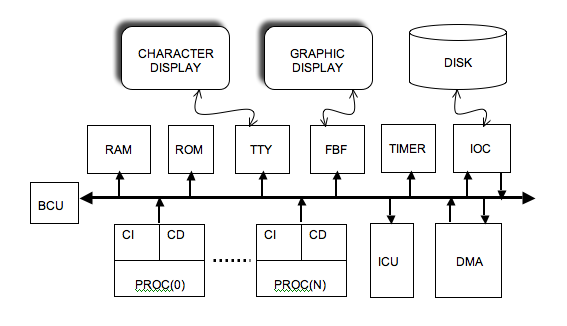
\includegraphics[width=11cm]{./tp8_topcell.png}\\[1ex]
  {\it Larchitecture que nous utiliserons sur ce TP est une à 4 processeurs.}
\end{center}

\subsection{Question C1}
L'utilisation du composant PibusBlockDevice impose d'augmenter la valeur du
time-out du composant PibusSegBcu à cause de son temps d'accès, celui ci étant
de l'ordre du millier, voire du million de cycles. Dans le cas de notre
architecture, le tems d'accès est défini par \texttt{IOC\_LATENCY}, qui est égal
à 1000 cycles.

Dans le cas où le time-out n'est pas modifié et garde sa valeur de 100 cycles,
tout transfert impliquant l'IOC échouerait. Il faut augmenter le time-out pour
le ramener dans l'ordre du millier de cycles.

\subsection{Question C2}
\begin{itemize}
  \item Le segment \texttt{seg\_ioc} est à l'adresse \texttt{0x92000000} est est
  de taille 32 octets.
  \item seg\_tty = 64 octets.
  \item seg\_icu = 128 octets.
  \item seg\_tim = 64 octets.
\end{itemize}

\subsection{Question C3}
\begin{itemize}
  \item On peut dénombrer 9 composants cibles : bcu, rom, ram, tty, fbf, timer,
  icu, dma \& ioc.
  \item On peut dénombrer 6 composants maîtres : proc[0..3], dma et ioc.
  \item L;élement à noter est qu'à l'instar du composant PibusDma,
  PibusBlockDevice est également un maître et une cible, pouvant recevoir et
  effectuer des requêtes.
\end{itemize}

\newpage

\subsection{Question C4}
\begin{minipage}{.5\textwidth}
  \begin{itemize}
    \item Les composants tty et timer ont une ligne d'interruption par processeur,
    dma et ioc ont respectivement leur propre ligne d'interruption. Le composant
    icu recoit donc en entrée 10 lignes d'interruptions :\\[1ex]
  \end{itemize}
\end{minipage}
\quad\quad
\begin{minipage}{.5\textwidth}
  \begin{tabular}{|c|c|}
    \hline
    \multicolumn{2}{|c|}{Entrées IRQ\_IN de l'ICU} \\ \hline
    IRQ\_IN[0] & DMA \\ \hline
    IRQ\_IN[1] & IOC \\ \hline
    IRQ\_IN[2] & TIMER[0] \\ \hline
    IRQ\_IN[3] & TTY[0] \\ \hline
    IRQ\_IN[4] & TIMER[1] \\ \hline
    IRQ\_IN[5] & TTY[1] \\ \hline
    IRQ\_IN[6] & TIMER[2] \\ \hline
    IRQ\_IN[7] & TTY[2] \\ \hline
    IRQ\_IN[8] & TIMER[3] \\ \hline
    IRQ\_IN[9] & TTY[3] \\ \hline
  \end{tabular}
\end{minipage}

\section{D) Code du boot}
\subsection{Question D1}
\begin{itemize}
  \item Dans le GIET, en l'absence de mémoire virtuelle, l'allocation des
  processus est faite statiquement. L'adresse de la pile par processeur (i) est
  alors alors : $seg\_stack[i] = seg\_stack\_base + i*seg\_stack\_size[i]$.
\end{itemize}

\subsection{Question D2}
Le routage des interruptions entrantes est effectué par le système
d'exploitation via le registre ICU\_MASK, qui permet de spécifier pour chaque
processeur quelles sont les lignes d'interruptions à acquitter.

\subsection{Question D3}
\begin{center}
  \begin{tabular}{|c|c|}
    \hline
    \multicolumn{2}{|c|}{Masques de routages \texttt{ICU\_MASK[i]}} \\ \hline
    IRQ\_TIM[0],IRQ\_TTY[0],IRQ\_DMA, IRQ\_IOC \hfill $\Rightarrow$ proc[0] & \texttt{0b0000001111} \\ \hline
    IRQ\_TIM[1],IRQ\_TTY[1] \hfill $\Rightarrow$ proc[1] & \texttt{0b0000110000} \\ \hline
    IRQ\_TIM[2],IRQ\_TTY[2] \hfill $\Rightarrow$ proc[2] & \texttt{0b0011000000} \\ \hline
    IRQ\_TIM[3],IRQ\_TTY[3] \hfill $\Rightarrow$ proc[3] & \texttt{0b1100000000} \\ \hline
  \end{tabular}
\end{center}

\section{E) Application logicielle de traitement d'image}
\subsection{Opérations du \texttt{main}}
\begin{itemize}
  \item Appel d'ioc\_read() : lecture d'une image sur le disque, copie de cette
  image dans buf\_in.
  \item Appel d'ioc\_completed() : attente de la fin du transfert.
  \item Traitement de l'image pixel par pixel  : application d'un seuil sur
  l'image, stocké dnas un tampon buf\_out.
  \item Appel de fb\_sync\_write() : affichage sur le framebuffer du tampon de
  sortie buf\_out.
\end{itemize}

\subsection{Quesiton E1}
La fonction \_ioc\_read() prend trois arguments :
\begin{itemize}
  \item \texttt{lba} : Adresse du 1er bloc sur le disque.
  \item \texttt{buffer} : Adresse du tampon mémoire où stocker les données lues.
  \item \texttt{count} : Nombre de blocs à transferer.
\end{itemize}
Cette fonction se bloque en attendant d'avoir accès à l'IOC avec la fonction
\_ioc\_get\_lock(). Cette fonction effectue une boucle en assembleur basée sur
LL/SC afin de garantir un accès atomique.

Une fois la ressource acquise,déclenche le transfert en écrivant dans le
registre
BLOCK\_DEVICE\_OP,

\subsection{Question E2}


\end{document}
